\chapter{Thesis Summary}


This thesis consists of five parts, with this introductory part being the first. The following three parts focus on research topics related to autonomous marine optimal control and path planning, as summarized in the block diagram shown in Figure~\ref{fig:uw_robot_planning_control}. Each chapter within these parts corresponds to a key component in the overall system, as illustrated:

\begin{itemize}
  \item Chapter IV presents the development of an \textit{UNav-Sim underwater robot simulator}, which provides a realistic environment for testing and validation.
  \item Chapter V focuses on an \textit{Entanglement Aware Tether Planner} that improves the robustness of the underwater vehicle tether management.
  \item Chapter VI presents a \textit{Visual Tracking Nonlinear Model Predictive Control (NMPC)} method for visually robust coverage.
  \item Chapters VII and VIII describe the learning and modeling of underwater dynamics via \textit{PINNs} and \textit{Gaussian Processes (GPs)}, respectively, which are integrated into the control and optimization modules.
\end{itemize}

The final part concludes with an overall summary and future research directions.

\begin{figure*}[t]
\centering
{\small
\begin{tikzpicture}[
    node distance=1.5cm and 1.8cm,
    block/.style={
        rectangle, 
        draw=TrajectoryBlue,         
        line width=0.8pt,   
        fill=TrajectoryBlue, 
        text=white, 
        text width=2.5cm, 
        align=center, 
        minimum height=1cm, 
        font=\bfseries,
        rounded corners=6pt
    },
    lbl/.style={
        rectangle, 
        draw=black, thick, 
        fill=white, 
        text=black, 
        text width=2.2cm, 
        align=center, 
        font=\bfseries\footnotesize, 
        minimum height=1cm
    },
    arrow/.style={-{Latex[width=2mm]}, thick, black},
    arrowlabel/.style={font=\bfseries\footnotesize, text=black, midway, above},
    bluearrow/.style={-{Latex[width=2mm]}, thick, TrajectoryBlue},
    bluearrowlabel/.style={font=\bfseries\footnotesize, text=TrajectoryBlue, midway, below}
]

% Top row labels
\node[lbl, xshift=-1.5cm] (C21a) {Chapter V\\Entanglement Aware\\Planner};
\node[lbl, right=of C21a] (C21b) {Chapter VI\\Visual Tracking\\NMPC};
\node[lbl, right=of C21b] (C1) {Chapter IV\\Underwater Robot\\Simulator};

% Second row
\node[block, below=of C21a, xshift=-0.3cm] (PathPlanner) {Path Planner};
\node[block, below=of C21b, yshift=-2pt] (Cost) {Cost};

\node[font=\bfseries\large] at ($(Cost.north)+(0.7cm,0.75cm)$) {MPC};

\node[below=of C1] (Sim) {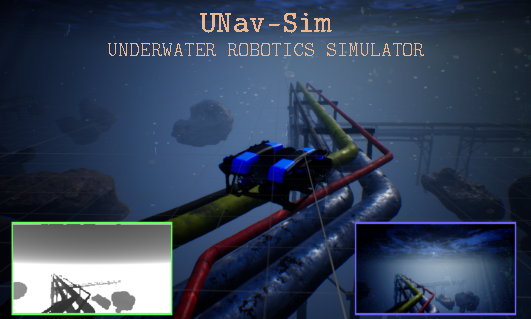
\includegraphics[width=4.0cm]{Phd_thesis/figures/UWRS_pipe.pdf}};

% Third row
\node[block, below=of PathPlanner] (Model) {Model};
\node[block, below=of Cost] (Optimizer) {Optimizer};

% Bottom labels
\node[lbl, below left=0.8cm and -0.5cm of Model] (C31) {Chapter VII\\Full Model\\Learning};
\node[lbl, below right=0.8cm and -0.5cm of Model] (C32) {Chapter VIII\\Residual Model\\Learning};

% Connections from labels
\draw[arrow] (C21a.south) -- ++(0,-1.5cm);
\draw[arrow] (C21b) -- (Cost);
\draw[arrow] (C1) -- (Sim);

% Main process flow
\draw[arrow] (PathPlanner) -- node[arrowlabel, xshift=-0.1cm] {reference} (Cost);

\draw[bluearrow] ($(Cost.east)+(0.6cm,0)$) -- (Cost.east);

\draw[TrajectoryBlue, thick] ($(Cost.east)+(0.61cm,0)$) -- ++(0,-0.9cm);





% Model learning connections
\draw[arrow] (C31) -- (Model);
\draw[arrow] (C32) -- (Model);

% Model to Optimizer
\draw[arrow] (Model) -- node[arrowlabel] {prediction} (Optimizer);

% Feedback from simulator to model
\draw[bluearrow] 
  ([xshift=2mm]Sim.west) -- 
  node[bluearrowlabel, xshift=2cm] {feedback} ++(-6.86,0)
  -- ++(0,-1)
  -- (Model.north);

% Performance metric
\draw[arrow, line width=1.6pt]
  (Cost.south) -- node[arrowlabel, left] {performance metric} ++(0,-1.5cm);

% Optimizer to output
\draw[arrow] (Optimizer.east) -- node[arrowlabel, below] {actions} ++(3,0) -- ++(0,0.5);

% Dashed enclosing box
\begin{scope}[on background layer]
    \coordinate (A) at ([xshift=-0.3cm,yshift=0.5cm]Cost.north west);
    \coordinate (B) at ([xshift=0.3cm,yshift=3.cm]Optimizer.north east);
    \coordinate (C) at ([xshift=0.3cm,yshift=-0.5cm]Optimizer.south east);
    \coordinate (D) at ([xshift=-3cm,yshift=-.5cm]Model.south east);
    \coordinate (E) at ([xshift=-0.3cm,yshift=2.07cm]Model.south west);
    \coordinate (F) at ([xshift=-0.3cm,yshift=-0.5cm]Cost.south west);
    \draw[dashed, thick]
        (A) -- (B) -- (C) -- (D) -- (E) -- (F) -- cycle;
\end{scope}

\end{tikzpicture}
}
\caption{Block diagram summarizing the key components and their interactions within the thesis framework. Each highlighted module corresponds to a specific chapter, illustrating how the development of the underwater robot simulator (Chapter 3), the entanglement-aware tether planner (Chapter 4), the visual tracking NMPC (Chapter 5), and the data-driven model improvements via PINNs and Gaussian Processes (Chapters 6 and 7) collectively contribute to advancing autonomous marine robotics optimal control.}
\label{fig:uw_robot_planning_control}
\end{figure*}













\section{Chapter IV}
\label{ch:simulator}
The development of reliable autonomous systems begins with the creation of a realistic simulation environment that supports rapid prototyping, synthetic data generation, and thorough testing of proposed algorithms. This is especially crucial in the context of underwater robotics, where field experiments are often expensive, logistically challenging, and time-consuming. Additionally, the absence of the Global Positioning System (GPS) underwater makes it difficult to obtain accurate ground-truth positioning, further underscoring the importance of simulation in the development cycle.


In this chapter, we address the critical need of visually realistic and customizable simulation tools in marine robotics. Compared to other robotics simulators, underwater simulators often suffer from limited rendering fidelity, poor underwater physics modeling, and weak integration with standard robotics tools such as ROS. To bridge this gap, we conducted a comprehensive survey of existing underwater simulators to identify their limitations and inform the design of a new tool.

To overcome these challenges, we introduce UNav-Sim, a novel, open-source underwater robotics simulator designed to support advanced autonomy and vision-based algorithms. UNav-Sim is the first underwater simulator to leverage Unreal Engine 5 (UE5) \cite{unreal} for high-fidelity visual environments while supporting essential robotics frameworks like ROS 2 and autopilot software. Built on top of AirSim \cite{airsim}, UNav-Sim enables rapid development and testing of underwater perception, navigation, and control algorithms. The framework includes a vision-based navigation stack and supports various sensor modalities, making it well-suited for both academic and industrial research. %Furthermore, we demonstrate UNav-Sim's applicability through a vision-based pipe-following task, integrating deep reinforcement learning, MPC, and ORB-SLAM for localization.




UNav-Sim has been widely adopted by the underwater robotics community, for realistic simulation and synthetic data generation. Future development will focus on expanding the suite of supported sensors, vehicle models, and customization underwater environments. 

With a robust simulation foundation in place, the next chapter shifts focus to a critical challenge in marine robotics: coverage path planning. We begin by addressing the limitations of traditional methods and introduce a novel framework tailored for safe and efficient inspection of complex underwater structures.


\section{Chapter V}
\label{ch:react}

Autonomous inspection of marine structures is one of the most common and critical applications of underwater robotics. These structures are typically deployed in harsh environments for extended periods, requiring frequent and reliable monitoring to ensure their integrity and performance. Traditional inspection methods using human divers are often costly, risky, and logistically challenging. In this context, coverage becomes a key requirement for effective inspection. While numerous coverage path planners (CPP) have been proposed in the literature, a critical limitation remains largely unaddressed: the risk of tether entanglement during inspection with tethered vehicles.
 
 In this chapter we present REACT, a novel real-time coverage path planning framework for tethered underwater vehicles, designed to enable safe and efficient inspection of underwater structures. Unlike traditional CPP frameworks that does not take into account risk entanglement, REACT integrates a fast geometry-based tether model utilizing signed distance fields (SDFs) to simulate the tether configuration in real time. By enforcing a maximum tether length constraint, REACT proactively prevents entanglement during mission execution.

The REACT framework operates by coupling this tether model with a MPC and an off-the-shelf CPP, facilitating online replanning and optimal trajectory tracking. The system has been validated in simulated pipe inspection tasks, where it demonstrated the ability to maintain full coverage while avoiding tether-related failures.

We also provide a comprehensive review of prior work in tether-aware planning, highlighting key limitations such as assumptions of 2D environments, reliance on offline computation, and lack of generalization to 3D scenarios. In contrast, REACT addresses these challenges by offering a scalable and adaptable solution suitable for complex and cluttered 3D underwater environments.

The chapter concludes with simulation results showing that, although REACT may incur a slight increase in inspection time, it ensures mission success by eliminating the risk of tether entanglement—making it essential for real-world underwater inspection tasks where safety and reliability are of utmost importance. 



\section{Chapter VI}
\label{ch:vtnmpc}

In this chapter, we address another critical challenge in coverage path planning: achieving visually robust inspection. We tackle this by incorporating perception objectives directly into the MPC framework. Specifically, we propose a novel Visual Tracking Nonlinear Model Predictive Control (VT-NMPC) autonomous wind turbine inspection framework designed to enable automated, safe, and efficient inspection of wind turbine blades using aerial robots. In contrast to traditional MPC-based approaches that track predefined position and heading trajectories, VT-NMPC introduces a surface-tracking paradigm, allowing the drone to follow inspection surfaces directly. This shift eliminates the need for precisely planned trajectories and enhances robustness to disturbances such as wind.

The proposed inspection framework consists of two key components:
\begin{itemize}
    
\item A novel global path planner that generates a distance-optimal sequence of surface regions to inspect across all turbine blades.

\item  A VT-NMPC controller that dynamically regulates the drone’s pose to maintain optimal distance and orientation relative to the blade surfaces, thereby ensuring high-resolution imaging while avoiding collisions.

\end{itemize}

The VT-NMPC cost function is designed to enforce visual inspection constraints — such as maintaining perpendicularity to the surface and respecting drone dynamics — making it inherently suited to the inspection task. This method reduces reliance on expert pilots, increases operational safety, and improves inspection quality.

The framework has been validated in both simulation and real-world tests on a custom-built drone platform. Results show that the proposed method achieves full blade coverage, demonstrates robustness to wind disturbances, and outperforms traditional trajectory-based MPC methods in terms of adaptability and visual inspection fidelity.

This chapter also reviews related work in automated drone-based inspection and details the complete pipeline from global path planning to real-time control. The open-sourced implementation further supports reproducibility and future research.



\section{Chapter VII}
\label{ch:pinc}


In this chapter, we address the challenge of learning accurate dynamic models for underwater vehicles—an essential requirement for precise trajectory tracking, and consequently, successful inspection and coverage. Developing reliable models for marine vehicles is particularly difficult due to the complex hydrodynamic interactions they encounter and the presence of uncertain or poorly known physical parameters, which makes deriving models from first principles highly challenging. While neural networks offer powerful function approximation capabilities and can model highly nonlinear behaviors such as vehicle dynamics, they are prone to overfitting, require large amounts of data, and often lack physical interpretability. To address these limitations, Physics-Informed Neural Networks (PINNs) have emerged as a promising approach by incorporating known physical laws—such as differential equations—directly into the learning process. This integration allows the model to remain consistent with physical constraints, improves generalization from limited data, and enhances interpretability.

Building on this, we introduce an application of Physics-Informed Neural Networks with Control (PINC) for modeling the dynamics of underwater vehicles. PINC combines data-driven neural network modeling with embedded physical laws to improve prediction accuracy and generalization over traditional purely data-driven models. The approach leverages control inputs and time as inputs to produce physically consistent state transitions, extending reliable predictions beyond the training domain.

The work details the design and evaluation of various PINC configurations, investigating effects of network architecture, loss functions, gradient weighting, and training strategies on model performance. The framework includes physics-based regularization terms that enforce dynamic consistency and integrates autoregressive prediction techniques to improve long-horizon forecasting accuracy.

Experimental validation on a simulated underwater vehicle demonstrates that PINC achieves superior predictive accuracy with minimal computational overhead compared to non-physics-informed baselines. Key improvements stem from residual connections, gradient normalization, adaptive learning rate scheduling, and careful hyperparameter tuning. Robustness to sensor noise was also assessed through noisy input injection during training.

The chapter contributes an open-source implementation of the PINC framework along with a synthetic underwater vehicle simulator for data generation, facilitating reproducibility and future research.



\section{Chapter VIII}
\label{ch:dfgp}

In this chapter, we address the challenge of disturbance modeling in marine robotics. Rather than learning the full system dynamics, we assume a known nominal model derived from first principles and explicitly learn the residual disturbances that affect system performance. These environmental disturbances can significantly degrade trajectory tracking for MPC. 

To address this, we propose a data-efficient approach using GPs to learn only the unmodeled effects. Recognizing that underwater disturbances evolve over multiple timescales, we introduce a novel Dynamic Forgetting Gaussian Process (DF-GP) framework. This method avoids costly hyperparameter retuning by combining the predictions of multiple GPs, each with tailored forgetting factors. The resulting disturbance estimates are used to update the predictive model within MPC, enhancing tracking accuracy across diverse underwater conditions.



%In this work, we learn the residuals of the system dynamics, assuming a known nominal model. This approach is more data-efficient since we only learn the unmodeled effects—specifically, disturbances impacting crucial aspects of the system. Particularly in underwater environments, disturbances vary over multiple timescales. To handle this, we propose a novel dynamic forgetting GP (DF-GP) methodology that compensates for operational disturbances without requiring hyperparameter retuning. This method optimally combines the predictions of several GPs designed with handcrafted forgetting factors, enabling precise disturbance estimation across varying timescales. The predicted disturbances update the model parameters within MPC, enabling a learning-based control framework that ensures accurate tracking in different underwater scenarios.

The key contributions of this study are:

\begin{itemize}
\item A learning-based MPC framework built upon a GP architecture that facilitates efficient disturbance learning of varying timescales along with unmodeled uncertainties.
\item An online adaptive framework that optimally weighs the predictions of multiple GPs with varying forgetting factors.
\item Validation of the proposed framework through extensive simulations and real-world experiments demonstrating improved performance.
\end{itemize}

Rigorous simulation and experimental results show a 25\% improvement in disturbance estimation and tracking performance, outperforming direct competitors.